\documentclass{llncs}
\usepackage{amsmath,amsfonts,wrapfig,graphicx,caption,url}
\usepackage{subcaption}
\usepackage[all]{xy}
\usepackage{tikz}
\usepackage{listings}
\usepackage{mathpartir}
\usepackage{mdframed}
\usepackage{proof}
\usetikzlibrary{automata,positioning}
\captionsetup{compatibility=false}
\newcounter{mycnt}
\pagestyle{plain}

\newcommand{\Nat}{\mathbb{N}}
\newcommand{\Z}{\mathbb{Z}}
\newcommand{\st}{\mathsf{st}}
\newcommand{\str}{\mathsf{str}}
\newcommand{\encb}{\mathit{eb}}
\newcommand{\EncB}{\mathit{EB}}
\newcommand{\encm}{\mathit{em}}
\newcommand{\CT}{\mathbb{CT}}
\newcommand{\dec}{\mathsf{dec}}
\newcommand{\enc}{\mathsf{enc}}

\begin{document}



\title{Verifiable Homomorphic Tallying for the Schulze Vote Counting
Scheme}

%
\author{Thomas Haines \inst{1} \and
      Dirk Pattinson\inst{2} \and Mukesh Tiwari \inst{2}}
\institute{NTNU, Norway \and
         Research School of Computer Science, ANU, Canberra}
\maketitle

\begin{abstract}
The encryption of ballots is crucial to maintaining integrity and 
anonymity in electronic voting schemes. It enables, amongst other 
things, each voter to verify that their encrypted ballot has been 
recorded as cast, by checking their ballot against a bulletin board. 

We present a verifiable homomorphic tallying scheme for the Schulze 
method that allows verification of the correctness of the count---on the 
basis of encrypted ballots---that only reveals the final tally. We 
achieve verifiability by using zero knowledge proofs for ballot 
validity and honest decryption of the final tally. Our formalisation 
takes places inside the Coq theorem prover and is based on an 
axiomatisation of cryptogtaphic primitives, and our main result is 
the correctness of homomorphic tallying. We then instantiate 
these primitives using an external library and show the feasibility 
of our approach by means of case studies.
\end{abstract}


\section{Introduction}

Secure elections are a balancing act between integrity and privacy:
achieving either is trivial but their combination is notoriously hard.
One of the key challenges faced by both paper based and electronic
elections is that results must substantiated with
verifiable evidence of their correctness while retaining the secrecy
of the individual ballot \cite{Bernhard:2017:PES}.  Technically, the
notion of ``verifiable evidence'' is captured by the term 
\emph{end-to-end (E2E) verifiability}, that is
\begin{itemize}
  \item every voter can verify that their ballot was cast as
  intended
  \item every voter can verify that their ballot was collected as
  cast
  \item everyone can verify final result on the basis of the
  collected ballots.
\end{itemize}
While end-to-end verifiability addresses the basic assumption that
no entity (software, hardware and participants) are inherently
trustworthy, ballot secrecy addresses the privacy problem.
Unfortunately, it appears as if coercion resistance is not achievable  
in the remote setting without relying on overly optimistic---to say the least---assumptions.
A weaker property called receipt-freeness captures the idea that an honest 
voter---while able to verify that their ballot was counted---is required to keep 
no information that a possible coercer could use to verify how that voter had voted.

End to end verifiability and the related notation of software independence~\cite{Rivest:2008:PTRS}
 have been claimed properties for many voting schemes.
 K{\"u}sters, Truderung and Vogt~\cite{Kusters:2010:CCS} 
 gave
 a cryptographic formulation whose value is highlighted by the attacks it revealed against established voting 
 schemes~\cite{Kusters:2012:SP}.

The combination of privacy and integrity can be realised using cryptographic techniques, where
encrypted ballots (that the voters themselves cannot decrypt) are
published on a bulletin board, and the votes are then processed, and
the correctness of the final tally is substantiated, using
homomorphic encryption \cite{Hirt:2000:ERF} and verifiable shuffling
\cite{Bayer:2012:EZK}. (Separate techniques exist to prevent ballot
box stuffing and to guarantee cast-as-intended.)
Integrity can then be guaranteed by means of Zero Knowledge Proofs
(ZKP),
first studied by Goldwasser, Micali, and Rackoff~\cite{Goldwasser:1985:STOC}.
Informally, a ZKP is a probabilistic and interactive proof where one
entity interacts with another such that the interaction provides
no information other than that the statement being proved is true with
overwhelming probability. 
Later results~\cite{Ben-Or:1988:CRYPTO,Goldreich:1991:ACM}
showed that 
all problems for which solutions can be efficiently verified have zero knowledge
proofs.


This paper addresses the problem of verifiable homomorphic tallying
for a preferential voting scheme, the Schulze Method. We show
how it can be implemented in a theorem prover to
guarantee both provably correct and verifiable counting on the basis
of encrypted ballots, relative to an axiomatisation of the
cryptographic primitives. We then obtain, via program extraction, a
provably correct implementation of vote counting, that we turn
into executable code by providing implementations of the primitives
based on a standard cryptographic library. We conclude by presenting
experimental results, and discuss trust the trust base, security and
privacy as well as the applicability of our work to real-world
scenarios. 

  \smallskip\noindent\emph{The Schulze Method.} The Schulze Method
  \cite{Schulze:2011:NMC} is a preferential, single-winner vote
  counting scheme that is gaining popularity due to its relative
  simplicity while retaining near optimal fairness
  \cite{Rivest:2010:OSW}.  
  A \emph{ballot} is a rank-ordered list of
  candidates where different candidates may be given the same rank.
  The protocol proceeds in two steps, and first computes the
  \emph{margin matrix} $m$, where $m(x, y)$ is the relative margin
  of $x$ over $y$, that is, the number of voters that prefer $x$
  over $y$, minus the number of voters that prefer $y$ over $x$. In
  symbols, given a collection $B$ of ballots, 
  \[ m(x, y) = \sharp\lbrace b \in B \mid x <_b y \rbrace
             - \sharp \lbrace b \in B \mid y <_b x \rbrace
  \]
  where $\sharp$ denotes cardinality, and $<_b$  is the preference
  relation encoded by ballot $b$. 
  We note that $m(x, y) = -m(y, x)$, i.e. the margin matrix is
  symmetric. In a second step, a \emph{generalised margin} $g$ is
  computed as the strongest path between two candidates
  \[ g(x,y) = \max \lbrace \str(p) \mid p \mbox{ path from $x$ to
  $y$} \rbrace \]
  where a path from $x$ to $y$ is simply a sequence $x = x_0, \dots,
  x_n = y$ of candidates, and the strength
  \[ \str(x_0, \dots, x_n) = \min \lbrace m(x_i, x_{i+1}) \mid 0
  \leq i < n
  \rbrace  \]
  is the lowest margin encountered on a path.
  Informally, one may think of the
  generalised margin $g(x, y)$ as transitive accumulated support for
  $x$ over $y$. We say that $x$ beats $y$ if $g(x,y) \geq g(y, x)$ and a
  winner is a candidate that cannot be beaten by anyone. 
  That is, $w$ is a \emph{winner} if $g(w, x) \geq g(x, w)$ for
  all other candidates $x$. Note that
  winners may not be uniquely determined (e.g. in the case where no
  ballots have been cast).

  In previous work \cite{Pattinson:2017:SVE} we have demonstrated
  how to achieve verifiability of counting plaintext ballots by
  producing a verifiable \emph{certificate} of the count, where
  ballot privacy and receipt freeness are not addressed. The
  certificate has two parts: The first part witnesses the
  computation of the margin matrix where each line of the
  certificate amounts to updating the margin matrix by a single
  ballot. The second part witnesses the determination of winners
  based on the margin matrix. In the first phase, i.e. the
  computation of the margin matrix, we perform the following
  operations for every ballot:
  \begin{enumerate}
    \item if the ballot is informal it will be discarded
    \item if the ballot is formal, the margin matrix will be
    updated
  \end{enumerate}
  The certificate then contains one line for each ballot and thus
  allows to independently verify the computation of the margin
  matrix. Based on the final margin matrix, the second part of
  the certificate presents verifiable evidence for the computation
  of winners. Specifically, if a candidate $w$ is a winner, it
  includes:
  \begin{enumerate}
    \item an integer $k$ and a path of strength $k$ from $w$ to any
    other candidate
    \item evidence, in the form of a co-closed set, of the fact that
    there cannot be a path of strength $> k$ from any other
    candidate to $w$.
  \end{enumerate}
  Crucially, the evidence of $w$ winning the election \emph{only}
  depends on the margin matrix. 
  We refer to \cite{Pattinson:2017:SVE} for details of the second
  part of the certificate as this will remain unchanged in the work
  we are reporting here.
    
   
\smallskip\noindent\emph{Related Work.} The paper that is closest to
our work is an algorithm for homomorphic counting for Single
Transferable Vote \cite{Benaloh:2009:SSC}. While single transferable
vote is arguably more complex that the Schulze Method, we have
demonstrated the viability of our approach by implementing it in a
theorem prover, and have extracted, and evaluated, an executable
based on the formal proof development. The idea of formalising
evidence for winning elections has been put forward (for plaintext
ballots) in \cite{Pattinson:2015:VCM}. For non-preferential
(plurality) voting, homomorphic tallying is now standard, and
implemented e.g. in the Helios electronic voting system
\cite{deMarneffe:2009:EUP} from Version 2.0 onwards, and is used
e.g. in public elections in Estonia \cite{Parsovs:2016:HTE}.

\section{Verifiable Homomorphic Tallying}
%\texttt{
%  Bullet points of content for reference and later deletion
%\begin{itemize}
%  \item general protocol, comparision with plaintext counting
%  \item two-phase structure: margin matrix, then winners with
%  winners as before: encryption commutes with margin computation
%  \item homomorphic computation of margin matrix, ballot
%  representation
%  \item computation of winners (as for plaintext)
%\end{itemize}
%}
The realisation of verifiable of homomorphic tallying that we are about to
describe follows the same two phases as the protocol: We first
homomorphically compute the margin matrix, and then compute
winners on the basis of the (decrypted) margin. The computation also
produces a verifiable certificate that leaks no information about
individual ballots other than the (final) margin matrix, which in
turn leaks no information about individual ballots if the number of
voters is large enough. As for counting of plaintext ballots, we
disregard informal ballots in the computation of the margin.
In accord with the two phases of computation, the certificate
consists of two parts: the first part evidences the correct
(homomorphic) computation of the margin, and the second part the
correct determination of winners. We describe both in detail.

\smallskip\noindent\emph{Format of Ballots.} In preferential voting
schemes, ballots are rank-ordered lists of candidates. For the
Schulze Method, we require that all candidates are ranked, and two
candidates may be given the same rank. That is, a ballot is most
naturally represented as a function $b: C \to \Nat$ that assigns a
numerical rank to each candidate, and the computation of the margin
amounts to computing the sum
\[ m(x, y) = \sum_{b \in B} \begin{cases} +1 & b(x) > b(y) \\ 0 &
b(x) = b(y) \\ -1 & b(x) < b(y) \end{cases} \]
where $B$ is the multi-set of ballots, and each $b \in B$ is a
ranking function $b: C \to \Nat$ over a (finite) set $C$ of
candidates. 

We note that this representation of ballots is not well suited for
homomorphic computation of the margin matrix as practically feasible
homomorphic encryption schemes do not support comparison operators
and case distinctions as used in the formula above. 

We instead represent ballots as matrices
$b(x, y)$ where $b(x, y) = +1$ if $x$ is preferred
over $y$, $b(x, y) = -1$ if $y$ is preferred over $x$ and $b(x, y) =
0$ if $x$ and $y$ are equally preferred.

While the advantage of the first representation is that each ranking
function is necessarily a valid ranking, the advantage of the matrix 
representation is that the computation of
the margin matrix is simple, that is
\[ m(c, d) = \sum_{b \in B} b(x, y) \]
where $B$ is the multi-set of ballots (in matrix form), and can
moreover be transferred to the encrypted setting in a straight
forward way: if ballots are matrices $e(x,y)$ where $e(x,y)$ is the
encryption of an integer in $\lbrace -1, 0, 1 \rbrace$, then
\begin{equation}\label{eqn:enc-mm}
\encm = \bigoplus_{\encb \in \EncB} \encb(x, y) 
\end{equation}
where $\oplus$ denotes homomorphic addition, $\encb$ is an encrypted
ballot in matrix form (i.e. decrypting $\encb(x, y)$ indicates
whether $x$ is preferred over $y$), and $\EncB$ is the multi-set of
encrypted ballots. The disadvantage is that we need to verify that a
matrix ballot is indeed valid, that is
\begin{itemize}
\item that the decryption of $\encb(x, y)$ is indeed one of $1, 0$ or
$-1$
\item that $\encb$ indeed corresponds to a ranking function.
\end{itemize}

\noindent
Indeed, to achieve verifiability, we not only need \emph{verify}
that a ballot is valid, we also need to \emph{evidence} its validity
(or otherwise) in the certificate.  

\smallskip\noindent\emph{Validity of Ballots.} By a plaintext
(matrix) ballot
we simply mean a function $b: C \times C \to \Z$,
where $C$ is the (finite) set of candidates. A 
plaintext ballot $b(x, y)$ 
is \emph{valid} if it is induced by a ranking function, i.e.
there exists a function $f: C \to \Nat$ such that $b(x, y) = 1$ if
$f(x) < f(y)$, $b(x, y) = 0$ if $f(x) = f(y)$ and $b(x, y) = -1$ if
$f(x) > f(y)$. A \emph{ciphertext (matrix) ballot} is a function
$\encb: C \times C \to \CT$ (where $\CT$ is a chosen set of
ciphertexts), and it is valid if its decryption,  i.e. the plaintext
ballot $b(x, y)  = \dec(\encb(x, y))$ is valid (where $\dec$ denotes
decryption).

For a plaintext ballot, it is easy to decide whether it is
valid (and should be counted) or not (and should be discarded). We
use shuffles (ballot permutations) to evidence the validity of
encrypted ballots. One observes that a matrix ballot is valid if and
only if it is valid after permuting both rows and columns with the
same permutation. That is, $b(x,y)$ is valid if and only if $b'(x,y)$
is valid, where
\[ b'(x,y) = b(\pi(x), \pi(y)) \]
and $\pi: C \to C$ is a permutation of candidates. (Indeed, if $f$
is a ranking function for $b$, then $f \circ \pi$ is a ranking
function for $b'$). As a consequence, we can evidence the validity
of a ciphertext ballot $\encb$ by
\begin{itemize}
  \item publishing a shuffled version $\encb'$ of $\encb$, that is
  shuffled by a secret permutation, together with
  evidence that $\encb'$ is indeed a shuffle of $\encb$
  \item publishing the decryption $b'$ of $\encb'$ together with
  evidence that $b'$ is indeed the decryption of $\encb'$.
\end{itemize}

\noindent
We use zero-knowledge proofs in the style of \cite{DBLP:conf/africacrypt/TereliusW10}
to evidence the correctness of the shuffle, and zero-knowledge
proofs of honest decryption \cite{DBLP:conf/crypto/ChaumP92} to evidence
correctness of decryption. This achieves ballot secrecy as
the (secret) permutation is never revealed.

In summary, the evidence of correct (homomorphic) counting starts
with an encryption of the zero margin $\encm$, and for each
ciphertext ballot $\encb$ contains
\begin{enumerate}
\item \label{it:shuff} a shuffle of $\encb$ together with a ZKP of 
correctness
\item decryption of the  shuffle, together with a ZKP of
correctness
\item \label{it:upd-marg} the updated margin matrix, if the decrypted ballot
was valid, and
\item the unchanged margin matrix, if the decrypted
ballot is not valid.
\setcounter{mycnt}{\value{enumi}}
\end{enumerate}
Once all ballots have been processed in this way, the certificate
determines winners and contains
winners by
\begin{enumerate}
\setcounter{enumi}{\value{mycnt}}
\item \label{it:pub-dm} the fully constructed margin, together with its decryption  
  and ZKP of honest decryption after counting all the ballots     
\item publishes the winner(s), together with evidence to substantiate the
    claim
\end{enumerate}


\smallskip\noindent\emph{Cryptographic primitives.}
We require an additively homomorphic cryptosystem to
compute the (encrypted) margin matrix according to Equation
\ref{eqn:enc-mm} (this implements Item \ref{it:upd-marg} above). All
other primitives fall into one of three categories.
\emph{Verification primitives} are used to syntactically define
the type of valid certificates. For example, when publishing the
decrypted margin matrix in Item \ref{it:pub-dm} above, we require
that the zero knowledge proof in fact evidences correct decryption.
To
guarantee this, we need a verification primitive that -- given
ciphertext, plaintext and zero knowledge proof -- verifies whether the supplied proof
indeed evidences that the given ciphertext corresponds to the given
plaintext. In particular, verification primitives are always boolean
valued functions. While verification primitives \emph{define} valid
certificates, \emph{generation primitives} are used to
\emph{produce} valid certificates. In the example above, we need a
decryption primitive (to decrypt the homomorphically computed
margin) and a primitive to generate a zero knowledge proof (that
witnesses correct decryption). Clearly verification and generation
primitives have a close correlation, and we need to require, for
example, that zero knowledge proofs obtained via a generation
primitive has to pass muster using the corresponding verification
primitive. 

The three primitives described above (decryption, generation of a
zero knowledge proof, and verification of this proof) already allow
us  to implement the entire protocol with exception of ballot
shuffling (Item \ref{it:shuff} above).  Here, the situation is more
complex. While existing mixing schemes (e.g. \cite{Bayer:2012:EZK}) permute 
an array of ciphertexts and produce a zero knolwedge proof that
evidences the correctness of the shuffle, our requirement dictates
that every row and colum of the (matrix) ballot is
shuffled with the \emph{same} (secret) permutation.  In other words,
we need to retain the identity of the permutation to guarantee that
each row and column of a ballot have been shuffled by the same
permutation.
We achieve this by
committing to a permutation using Pedersen's commitment scheme
\cite{Pederson}.
In a nutshell, the Pedersen commitment scheme has the following properties. 
\begin{itemize}
\item Hiding: the commitment reveals no information about the
permutation
\item Binding: no party can open the commitment in more  
	 	than one way, i.e. the commitment is to one permutation only. 
\end{itemize}

\noindent
A combination of Pedersen's commitment scheme 
with a zero knowledge proof leads to a similar two step protocol, also known 
as commitment-consistent proof of shuffle \cite{Wikstrom:2009:CPS}.

\begin{itemize}
\item Commit to a secret permutation and publish the commitment (hiding).
\item Use a zero knowledge proof to show that shuffling has used 
      the same permutation which we committed to in previous step (binding).
\end{itemize}  

\noindent
This allows us to witness the validity (or otherwise) of a ballot by generating a 
permutation $\pi$ which is used to shuffle every row and column of the ballot.
We hide $\pi$ by committing it using Pedersen's 
commitment scheme 
and record the commitment $c_{\pi}$ in the certificate. However, for the binding step, rather 
than opening $\pi$ we generate a zero knowledge proof, $zkp_{\pi}$, 
using $\pi$ and $c_{\pi}$, which can 
be  used to prove that $c_{\pi}$ is indeed the commitment to some permutation
used in the (commitment consistent) shuffling 
 without being opened \cite{Wikstrom:2009:CPS}. We can now use the
 permutation that we have committed to for 
shuffling each row and column of a ballot, and evidence the
correctness of the shuffle via a zero knowledge proof.
%
To evidence validity (or otherwise) of a (single) ballot, we
therefore:
\begin{enumerate}
  \item generate a (secret) permutation and publish a commitment to this
  permutation, together with a zero knowledge proof that evidences commitment
  to a permutation
  \item for each row of the ballot, publish a shuffle of the row with
  the permutation committed to, together with a zero knowledge proof
  that witnesses shuffle correctness
  \item for each column of the row shuffled ballot, publish a
  shuffle the column, also together with a zero knowledge proof of
  correctness 
  \item publish the decryption the ballot shuffled in this way, together with a
  zero knowledge proof that witnesses honest decryption
  \item decide the validity of the ballot based on the decrypted
  shuffle.
\end{enumerate}

\noindent
The cryptographic primitives needed to implement this again fall
into the same classes. To define validity of certificates, we need
verification primitives
\begin{itemize}
  \item to decide whether a zero knowledge proof evidences that a
  given commitment indeed commits to a permutation 
  \item to decide whether a zero knowledge proof evidences the
  correctness of a shuffle relative to a given permutation
  commitment.
\end{itemize}

\noindent
Dual to the above, to generate (valid) certificates, we need the
ability to
\begin{itemize}
  \item generate permutation commitments and accompanying zero
  knowledge proofs that evidence commitment to a permutation
  \item generate shuffles relative to a commitment, and zero
  knowledge proofs that evidence the correctness of shuffles.
\end{itemize}

\noindent
Again, both need to be coherent in the sense that the zero knowledge
proofs produced by the generation primitives need to pass
validation. In summary, we require an additively homomorphic
cryptosystem that implements the following:

\begin{description}
\item[Decryption Primitives.]
  decryption of a ciphertext, creation and verification of
  honest decryption zero knowledge proofs.
\item[Commitment Primitives.]
  generating permutations, creation and verification of commitment
  zero knowledge proofs
\item[Shuffling Primitives.]
  commitment consistent shuffling, creation and verification of
  commitment consistent zero knowledge shuffle proofs 
\end{description}

\smallskip\noindent\emph{Witnessing of Winners.}
Once all ballots are counted, the computed margin is decrypted, and
winners (together with evidence of winning) are computed using 
plaintext counting. We discuss this part only briefly, for completness,
 as it is identicial to the existing work on plaintext counting
\cite{Pattinson:2017:SVE}. For each of the winners $w$ and each
candidate $c$ we publish
\begin{itemize}
\item a natural number $k(w, x)$
\item a path $w = x_0, \dots, x_n = x$ of strength $k$
\item a set $C(w, x)$ of pairs of candidates that is $k$-coclosed
and contains $(x, w)$
\end{itemize}
where a set $S$ is  $k$-coclosed if for all $(x,z) \in C$ we have
that $m(x, z) < k$ and either $m(x, y) < k$ or $(y,z) \in S$ for
all candidates $y$.  Informally, the first requirement ensures that
there is no direct path (of length one) between a pair $(x, z) \in
S$ ,and the second requirement ensures that for an element $(x, z)
\in S$, there cannot be a path that connects $x$ to an intermediate
node $y$ and then (transitively) to $z$ that is of strength $\geq
k$. 
We refer to \emph{op.cit.} for the (formal)
proofs of the fact that existence of co-closed sets witnesses the
winning conditions. 
  



\section{Realisation in a Theorem Prover} \label{sec:realisation}
%\texttt{
%  Bullet points of content for reference and later deletion
%\begin{itemize}
%  \item Axiomatisation of the cryptographic primitives
%  \item correctness proof modulo correct crypto
%  \item describe certificates and how to check them
%  \item show that ``certificates certify''
%\end{itemize}}

%(* Remember the question. Why abstract because our purpose is to 
%   audit the election, and not verify crypto primitives ? *) 
We formalise homomorphic tallying for the Schulze Method inside the
Coq theorem prover \cite{Bertot:2004:ITP}. Apart from supporting an
expressive logic and (crucial for us) dependent inductive types, Coq
has a well developed extraction facility that 
we use to extract proofs into OCaml programs. Indeed, our basic
approach is to first formally define the notion of a valid
certificate, and then prove that a valid certificate can be obtained
from any set of (encrypted) ballots. Extracting this proof as a
programme, we obtain an executable that is correct by construction. 

The purpose of this paper is not to verify cryptographic primitives, 
but use them as a tool to construct evidence which can be used 
to audit and verify the outcome during different phase 
of election. Here, we treat them as abstract entities and assume
axioms about them inside Coq.
In particular, we assume the existence of functions that implement
each of the primitives described in the previous section, and
postulate natural axioms that describe how the different primitives
interact. As a by-product, we obtain an axiomatisation of a
cryptographic library that we could, in a later step, verify the
implementation of a cryptosystem against.  In particular, this
allows us to not commit to any particular cryptosystem in particular
(although our development, and later instantiation, is geared
towards El Gamal \cite{DBLP:conf/crypto/Gamal84}).

The first part of our formailsation concerns the cryptographic
primitives that we collect in a separate module. Below is an example
of the generation / verification primitives for decryption, together
with coherence axioms.
\begin{lstlisting}[frame=single,basicstyle=\ttfamily\footnotesize]
Variable decrypt_message: 
  Group -> Prikey -> ciphertext ->  plaintext.

Variable construct_zero_knowledge_decryption_proof:
  Group -> Prikey -> ciphertext -> DecZkp.

Axiom verify_zero_knowledge_decryption_proof:
  Group -> plaintext -> ciphertext -> DecZkp -> bool.

Axiom honest_decryption_from_zkp_proof: forall group c d zkp, 
 verify_zero_knowledge_decryption_proof group d c zkp = true 
 -> d = decrypt_message grp privatekey c.
 
Axiom verify_honest_decryption_zkp (group: Group):
  forall (pt : plaintext) (ct : ciphertext) (pk : Prikey),
  (pt = decrypt_message group pk ct) ->
  verify_zero_knowledge_decryption_proof group pt ct 
  (construct_zero_knowledge_decryption_proof group pk ct) 
  = true.
  

\end{lstlisting}
  
\noindent
The difference between the keyword \texttt{Variable} and \texttt{Axiom}
is purely syntactic, and in our case, used as a convenience for 
extraction. In
the above, the first two functions, \texttt{decrypt\_message} and
\texttt{construct\_zero\_knowledge\_decryption\_proof} are
\emph{generation} primitives, whereas 
\texttt{verify\_zero\_knowledge\_decryption\_proof} is a
\emph{verification} primitive. We have two coherence axioms. The
first says that if the verification of a zero knowledge proof of
honest decryption suceeds, then the ciphertext indeed decrypts to
the given plaintext. The second stipulates that generated zero
knowledge proofs indeed verify. 

For ballots, we assume a type \texttt{cand} of candidates, and
represent plaintext and encrypted ballots as two-argument functions
that take plaintext, and ciphertexts, as values. 
\begin{lstlisting}[frame=single,basicstyle=\ttfamily\footnotesize]
    Definition pballot := cand -> cand -> plaintext.
    Definition eballot := cand -> cand -> ciphertext.
\end{lstlisting}

\iffalse
=======
\end{lstlisting}
\textbf{Coherence Axioms:}
\begin{lstlisting}[frame=single,basicstyle=\ttfamily\footnotesize]
Axiom verify_honest_decryption_zkp :
 forall (group : Group) (pt : plaintext) 
 (ct : ciphertext) (privatekey : Prikey) 
 (H : pt = decrypt_message group privatekey ct),
 verify_zero_knowledge_decryption_proof
  group pt ct (construct_zero_knowledge_decryption_proof
                group privatekey ct) = true.
\end{lstlisting}
    
%\footnote{DP: separate ballots from decryption. Give example of ZKP
%generation / verification}.
%
%{\tt --------------------------------------------------------------
%}

\noindent
We represent plain text by the Coq data
type of integers (as this is the information that is to be
encrypted), but leave ciphertext as an abstract type, to be
instantiated later. Honest decryption ZKP construction primitive
takes a element of Group, private key, cipher text
and returns element of DecZkp (abstract type which represents 
decryption zero knowledge proof). 
An element of a \texttt{Group} is 
a triplet of large prime number, group generator and public key. 
Honest decryption verification primitive verifies the claim about 
constructed zero knowledge proof, i.e. it takes the group, 
plaintext, ciphertext, decryption zero knowledge proof, and returns true 
or false. A true value means claim is legitimate, otherwise bogus.      
For ballots, we assume a type \texttt{cand} of candidates, and
represent plaintext and encrypted ballots as two-argument functions
that take integers, and ciphertexts, as values. 

\begin{lstlisting}[frame=single,basicstyle=\ttfamily\footnotesize]
 Definition plaintext := Z.
 Variable ciphertext : Type.
 Definition pballot := cand -> cand -> plaintext.
 Definition eballot := cand -> cand -> ciphertext.
\end{lstlisting}
 
>>>>>>> b8a2587d059ddd944603131ec4d821130c95dc5d
\fi
  \noindent
  We now turn to the representation of certificates, and indeed to the
  definition of what it means to (a) count encrypted votes correctly
  according to the Schulze Method, and (b) produce a verifiable
  certificate of this fact. At a high level, we split the counting
  (and accordingly the certificate) into \emph{states}. This gives
  rise to a (dependent, inductive) type \texttt{ECount}, parameterised
  by the ballots being counted.

  \begin{lstlisting}[frame=single,basicstyle=\ttfamily\footnotesize]
  Inductive ECount (group : Group) (bs : list eballot) : 
    EState -> Type
  \end{lstlisting}

  \noindent
  Given a list \texttt{bs} of ballots, \texttt{ECount bs} is a
  dependent inductive type. In this case, given a state of counting
  (i.e. an inhabitant \texttt{estate} of \texttt{EState}), the type level application
  \texttt{ECount bs estate} is the \emph{type of evidence that proves
  that \texttt{estate} is a state of counting that has been reached
  according to the method}.  The states itself are represented by
  the type \texttt{EState}
where
\begin{itemize}
 \item \texttt{epartial} represents a partial state of counting,
 consisting of the homomorphically computed margin so far, the ist
 of uncounted ballots and the list of invalid ballots encountered so
 far
 \item \texttt{edecrypt} represents the final decrypted margin
 matrix, and 
 \item \texttt{ewinners} is the final determination of winners. 
\end{itemize}
This is readily translated to the following Coq code:
\begin{lstlisting}[frame=single,basicstyle=\ttfamily\footnotesize]
Inductive EState : Type :=
 | epartial : (list eballot * list eballot) ->
              (cand -> cand -> ciphertext) -> EState
 | edecrypt : (cand -> cand -> plaintext) -> EState
 | ewinners : (cand -> bool) -> EState.
\end{lstlisting}

\noindent
The constructors of \texttt{EState} then allow us to move from one
state to the next, under appropriate conditions that guaratnee
correctness of the count.

The first constructor, \texttt{Ecax} kick-starts the count, and
ensures that 
\begin{itemize}
  \item all ballots are initially uncounted
  \item margin matrix is an encryption of the zero matrix
\end{itemize}
The first constructor, as well as all the others, require
\begin{description}
  \item[state data] here, the list of uncounted and invalid ballots,
  and the encrypted homomorphic margin
  \item[verification data] a zero knowledge proof that the encrypted
  homomorphic margin is indeed an encryption of the zero margin
  \item[correctness constraints] here, the constuctor may only be applied if
  the list of uncounted ballots is equal to the list of ballots
  cast, and the fact that the zero knowledge proofs indeed verify
  that the intitial margin matrix is identically zero.
\end{description}

\noindent
The main difference between the correctness condition, and the
verification data is that the former can be simply be inspected
(here by comparing lists) whereas the latter requires additional
data (here  in the form of a zero knowledge proof).

The translation of high level representation into Coq representation
is now easy, and we arrive at the following Coq code.
\begin{lstlisting}[frame=single,basicstyle=\ttfamily\footnotesize]
ecax (us : list eballot) (encm : cand -> cand -> ciphertext)
 (decm : cand -> cand -> plaintext) 
 (zkpdec : cand -> cand -> DecZkp) :
 us = bs -> (forall c d : cand, decm c d = 0) -> 
 (forall c d, verify_zero_knowledge_decryption_proof 
   group (decm c d) (encm c d) (zkpdec c d) = true) -> 
 ECount group bs (epartial (us, []) encm)
\end{lstlisting}


\noindent
The constructor \texttt{ecvalid} represents the effect of counting a
valid ballot. Here the crucial aspect is that validity needs to be
evidenced. As before, we have:
\begin{description}
  \item[state data] as before, the list of uncounted and invalid
  ballots, the homomorphic margin, but additionally evidence that
  the previous state has been obtained correctly
  \item[verification data]
  a commitment to a (secret) permutation, a row permutation of the
  ballot being counted, and a column permutation of this, and a
  decryption of the row- and column permuted ballot (all with
  accompanying zero knowledge proofs)
  \item[correctness constraints] all the zero knowledge proofs
  verify, the new margin is the homomorphic addition of the previous
  margin and the counted ballot, and the decrypted (shuffled)
  ballot is indeed valid.
\end{description}


\noindent
We elide the description of the third constructor that is applied
when an invalid ballot is being encountered (the only
difference is that the margin matrix is not being updated). 
Counting finishes when there are no more uncounted ballots, in
which case the next step is to publish the decrypted margin matrix.
Also here, we have
\begin{description}
  \item[state data] the decrypted margin matrix, plus evidence
  that a state with no more uncounted ballots has been obtained
  correctly
  \item[verification data] a zero knowledge proof that demonstrates
  honest decryption of the final margin matrix
  \item[correctness constraints] the given zero knowledge proof
  verifies, i.e. the given decrypted margin is indeed the decryption
  of the (last) homomorphically computed margin matrix.
\end{description} 

\noindent
The last constructor finally declares the winners of the election,
and we have:
\begin{description}
  \item[state data] a function \texttt{cand -> bool} that determines
  winners, plus evidence of the fact that the decrypted final margin
  matrix has been obtained correctly
  \item[verification data] 
   paths and co-closed sets that evidence the correctness of the
   function above
 \item[correctness constraints] that ensure that the verification
 data verifies the winners given by the state data.
\end{description}
This last part is identical to our previous formalisation of the
Schulze Method (for plaintext ballots), and we refer to 
\cite{Pattinson:2017:SVE} for more details.


\section{Correctness by Construction and Verification}
\label{sec:correct}

In the previous section, we have presented a data type that
\emph{defines} the notion of a verifiably correct count of the
Schulze Method, on the basis of encrypted ballots. To obtain an
executable that in fact \emph{produces} a verifiable (and provably
correct) count, we can proceed in either of two ways:
\begin{enumerate}
  \item implement a function that -- give a list \texttt{bs} of
  ballots -- produces a boolean function \texttt{w} (for winners) and an
  element of the type \texttt{ECount bs (winners w)}. This gives
  both the eletion winners (\texttt{w}) as well as evidence (the
  element of the \texttt{ECount} data type).
  \item to prove that for every set \texttt{bs} of encrypted
  ballots, we have a boolean function \texttt{w} and an inhabitant
  of the type \texttt{ECount bs (winners w)}.
\end{enumerate}

\noindent
Under the proofs-as-programs interpretation of constructive type
theory, both amount to the same. We chose the latter approach, and
our first main theorem formally states that all elections can be
counted according to the Schulze Method (with encrypted ballots),
i.e. a winner can always be found. Formally, our main theorem takes
the following form:
\begin{lstlisting}[frame=single,basicstyle=\ttfamily\footnotesize]
Lemma pschulze_winners (group : Group) 
 (bs : list eballot) : existsT (f : cand -> bool), 
 ECount group bs (ewinners f).
\end{lstlisting}

\noindent
The proof proceeds by successively building an inhabitant of
\texttt{EState} by homomorphically computing the margin matrix, then
decrypting and determining the winners. Within the proof, we use
both generation primitives (e.g. to construct zero knowledge proofs)
and coherence axioms (to ensure that the zero knowledge proofs
indeed verify). 

The correctness of our entire approach stands or falls with the
correct formalisation of the inductive data type \texttt{ECount}
that is used to determine the winners of an election counted
according to the Schulze Method. While one can argue that the data
type itself is transparent enough to be its own specification,
the cryptographic aspect makes things slightly more complex. For
example, it appears to be credible that our mechanism for
determining validity of a ballot is correct -- however we have not
given proof of this. Rather than scrutinising the details of the
construction of this data type, we follow a different approach: we
demonstrate that homomorphic counting always yields the same results
as plaintext counting, where plaintext counting is already verified
against its specification. Plaintext counting has been formalised,
and verified, in the precursor paper \cite{Pattinson:2017:SVE}. This
correspondence has two directions, and both assume that we are given
two lists of ballots that are the encryption (resp. decryption) of
one another. 

The first theorem, \texttt{plaintext\_schulze\_to\_homomorphic}, reproduced below shows
that every winner that can be determined using plaintext counting
can also be evidenced on the basis of encrypted ballots. The
converse of this is established by 
Theorem \texttt{homomorphic\_schulze\_to\_plaintext}.

\begin{lstlisting}[frame=single,basicstyle=\ttfamily\footnotesize]
  Lemma plaintext_schulze_to_homomorphic 
   (group : Group) (bs : list ballot): 
   forall (pbs : list pballot) (ebs : list eballot) 
   (w : cand -> bool), (pbs = map (fun x => (fun c d => 
   decrypt_message group privatekey (x c d))) ebs) ->
   (mapping_ballot_pballot bs pbs) -> 
   Count bs (winners w) -> ECount group ebs (ewinners w).
      
  Lemma homomorphic_schulze_to_plaintext 
   (group : Group) (bs : list ballot):
   forall (pbs : list pballot) (ebs : list eballot) 
   (w : cand -> bool) (pbs = map (fun x => (fun c d => 
   decrypt_message group privatekey (x c d))) ebs) ->
   (mapping_ballot_pballot bs pbs) ->
   ECount grp ebs (ewinners w) -> Count bs (winners w).
\end{lstlisting}

\noindent
The theorems above feature a third type of ballot that is the basis
of plaintext counting, and is a simple ranking function of type
\texttt{cand -> Nat}, and the two hypotheses on the three types of
ballots ensure that the encrypted ballots (\texttt{ebs}) are in fact
in alignment with the rank-ordered ballots (\texttt{bs}) that are
used in plaintext counting. 
The proof, and indeed the formulation, relies on an inductive data
type \texttt{Count} that can best be thought of as a plaintext
version of the inductive type  \texttt{ECount} given here.
Crucially, \texttt{Count} is verified against a formal specification
of the Schulze Method. Both theorems are proven by induction on the
definition of the respective data types, where the key step is to
show that the (decrypted) final margins agree. The key ingredient
here are the coherence axioms that stipulate that zero knowledge
proofs that verify indeed evidence shuffle and/or honest decryption.



\section{Extraction and Experiments} \label{sec:extract}

As already mentioned, we are using  the Coq extraction
mechanism\cite{Letouzey:2003:NEC}  to extract programs from
existence 
proofs\footnote{https://github.com/mukeshtiwari/EncryptionSchulze/tree/master/code/Workingcode}. In particular, we extract the proof of the Theorem
\texttt{pschulze\_winners}, given in Section \ref{sec:correct} to a
program that delivers not only provably correct counts, but also
verifiable evidence.  Give a set of encrypted ballots and a \texttt{Group}
that forms the basis of cryptographic operations, we obtain a program that
delivers not only a set of winners, but additionally independently  verifiable
evidence of the correctness of the count. 

Indeed, the entire formulation of our data type, and the split into
state data, verification data, and correctness constraints, has been
geared towards extraction as a goal. Technically, the verification
conditions are \emph{propositions}, i.e. inhabitants of Type
\emph{Prop} in the terminology of Coq, and hence erased at
extraction time. This corresponds to the fact that the assertions
embodied in the correctness constraints can be verified with minimal
computational overhead, given the state and the verification data.
For example, it can simply be verified whether or not a zero
knowledge proof indeed verifies honest decryption by running
it through a verifier.  On the other hand, the zero knowledge proof
itself (which is part of the verification data) is crucially needed
to be able to verify that a plaintext is the honest decryption of a
ciphertext, and hence cannot be erased during extraction.
Technically, this is realised by formulating both state and
verification data at type level (rather than as propositions). 

As we have explained in Section \ref{sec:realisation}, the formal
development does not pre-suppose any specific implementation of the
cryptographic primitives, and we assume the existence of
cryptographic infrastructure. From the perspective of extraction,
this produces an executable with ``holes'', i.e. the cryptographic
primitives need to be supplied to fill the holes and indeed be able
to compile and execute the extracted program.  

To fill this hole, we implement the cryptoraphic primitives with
help of the UniCrypt library\cite{LocherH14}.
UniCrypt is a freely available library, written in Java,  that provides nearly all of
the required functionality, with the exception of honest decryption
zero knowledge proofs.  We extract our proof development into OCaml
and use Java/OCaml bindings~\cite{OCamlJava} to make the UniCrypt
functionality available to our OCaml program. Due to differences
in the type structure between Java and OCaml, mainly in the context
of sub-typing, this was done in the form of an OCaml wrapper around
Java data structures. 
 After instantiating the  
 cryptographic primitives in the extracted OCaml code with wrapper
 code that calls UniCrypt
 we tested the executable on a three candidate elections between
 candidates \texttt{A}, \texttt{B} and \texttt{C}.
 The computation produces a tally sheet that is schematically given
 below:
 it is trace of computation which can be used as a checkable record to verify
 the outcome of election. We elide the cryptographic detail, e.g.
 the concrete representation of zero knowledge proofs.
 A certificate
 is be obtained from the type \texttt{ECount} where the head
 of the certificate corresponds to the base case of the inductive
 type, here \texttt{ecax}. Below, \texttt{M} is encrypted margin
 matrix, \texttt{D} is its decrypted equivalent, required to be
 identically zero, and \texttt{Z} represents a matrix of zero
 knwoledge proofs, each establishing that the \texttt{XY}-component
 of \texttt{M} is in fact an encryption of zero. All these matrices
 are indexed by candidates and we display these matrices by listing
 their entries prefixed by a pair of candidates, e.g. the ellipsis
 in \texttt{AB(...)} denotes the matrix entry at row \texttt{A} and
 column \texttt{B}.

 {\small
 \begin{verbatim}
 M: AB(rel-marg-of-A-over-B-enc), AC(rel-marg-of-A-over-C-enc), ... 
 D: AB(0)                       , AC(0)                       , ...
 Z: AB(zkp-for-rel-marg-A-B)    , AC(zkp-for-rel-marg-A-B)    , ...
 \end{verbatim}}
 
 \mbox{}\\[-5ex]
 Note that one can verify the fact that the initial encrypted margin
 is in fact the zero margin by just verifying the zero knowledge
 proofs. Successive entries in the certificate will generally be
 obtained by counting valid, and discarding invalid ballots. If a
 valid ballot is counted after the counting commences, the
 certificate would continue by exhibiting the state and verification
 data contained in the \texttt{ecvalid} constructor which can be
 displayed schematically as follows:

 {\small\begin{verbatim}
 V: AB(ballot-entry-A-B) , AC(ballot-entry-A-C), ...
 C: permutation-commitment
 P: zkp-of-valid-permutation-commitment
 R: AB(row-perm-A-B)     , AC(row-perm-A-C)    , ...
 RP: A(zkp-of-perm-row-A), B(zkp-of-perm-row-B), ... 
 C: AB(col-perm-A-B),      AC(col-perm-A-C)    , ...
 CP: A(zkp-of-perm-col-A), B(zkp-of-perm-col-C), ...
 D: AB(dec-perm-bal-A-B) , AC(dec-perm-bal-A-C), ...
 Z: AB(zkp-for-dec-A-B)  , AC(zkp-for-dec-A-C) , ...
 M: AB(new-marg-A-B)     , AC(new-marg-A-C)    , ...
 \end{verbatim}}

 \mbox{}\\[-5ex]
 Here \texttt{V} is the list of ballots to be counted, where we only
 diplay the first element. We
 commit to a permutation and validate this commitment with a zero
 knowledge proof, here given in the second and third line, prefixed
 with \texttt{C} and \texttt{P}. The following two lines are a row
 permutation of the ballot \texttt{V}, together with a zero
 knowledge proof of correctness of shuffling (of each row) with
 respect to the permutation committed to by \texttt{C} above. The
 following two lines achieve the same for subsequently permuting the
 columns of the (row permuted) ballot. Finally, \texttt{D} is the
 decrypted permuted ballot, and \texttt{Z} a zero knowledge proof of
 honest decryption. We end with an updated homomorphic margin
 matrix \texttt{M}. Again, we note that the validity of the
 decrypted ballot can be checked easily, and validating zero
 knowledge proofs substantiate that the decrypted ballot is indeed a
 shuffle of the original one. Homomorphic addition can simply be
 re-computed.

 The steps where invalid ballots are being detected is similar, with
 the exception of not updating the margin matrix. Once all ballots
 are counted, the only applicable constructor is \texttt{ecdecrypt},
 the data content of which would continue a certificate
 schematically as follows:

 {\small\begin{verbatim}
 V: []
 M: AB(fin-marg-A-B), AC(fin-marg-A-C), ...
 D: AB(dec-marg-A-B), AC(dec-marg-A-C), ...
 Z: AB(zkp-dec-A-B) , AC(zkp-dec-A-C) , ...
 \end{verbatim}}

 \mbox{}\\[-5ex]
 Here the first line indicates that there are no more ballots to be
 counted, \texttt{M} is the final encrupted margin matrix,
 \texttt{D} is its decryption and \texttt{Z} is a matrix of zero
 knowledge proofs verifying the correctness of decryption.

 The certificate would end with the determination of winners based
 on the encrypted margin, and would end with the content of the
 \texttt{ecfin} constructor

 {\small\begin{verbatim}
 winning: A, <evidence that A wins against B and C>
 losing:  B, <evidence that B loses against A and C>
 losing:  C, <evidence that C loses against A and B>
 \end{verbatim}}

 \mbox{}\\[-5ex]
 where the notion of evidence for winning and losing is as in the
 plaintext version of the protocol \cite{Pattinson:2017:SVE}.

\begin{wrapfigure}{R}{7.4cm}
\centering
\vspace*{-1cm}
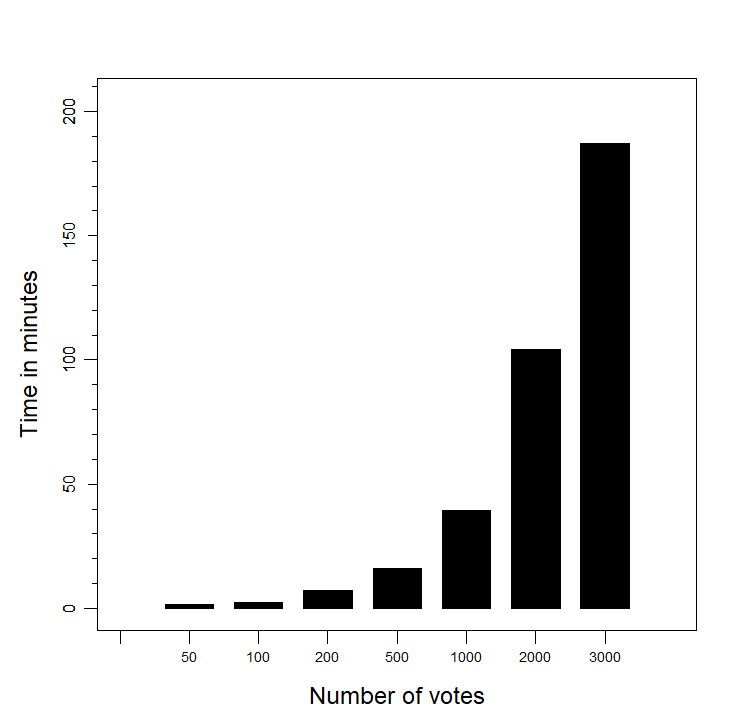
\includegraphics[scale=0.40]{PlotVer3.png}
\vspace*{-1cm}
\end{wrapfigure}
 We note that the schematic persentation of the certificate above is
 nothing but a representation of the data contained in the extracted
 type \texttt{ECount} that we have chosen to present schematically.
 Concrete certificates can be inspected with the accompanying proof
 development, and are obtained by simply implementing datatype to
 string conversion on the type \texttt{ECount}.

%%% DP: I don't understand this ... ? %%%%

The fact that the certificate was produced using formally verified
code implies that (modulo correctness of the implementation of the
cryptographic primitives) all certificates necessarily verify.
\emph{Verifiability} ensures that external stakeholders can convince
themselves in a hardware/software independent way of the correctness
of the count, whereas producing certiciates using \emph{verified}
code ensures that election authorities always produce correct, and
verifiable, results.


We have run our experiment on an  Intel  i7  2.6  GHz  Linux  desktop  computer
with  8GB  of  RAM for three candidates and randomly generated ballots. The 
highest amount of ballot we counted was 10,000 (not included in graph), and 
it ran for 25 hours. Clearly, it is not very efficient, and the reason we 
suspect is a lot of communication between OCaml runtime system 
and Java run time system.

\section{Analysis}

\noindent\emph{Summary.} The main contribution of our formalisation is that of independently
verifiable \emph{evidence} for a set of candidates to be the winners
of an election counted according to the Schulze method. Our main
claim is that that our notion of evidence is both safeguarding the
privacy of the individual ballot (as the count is based on encrypted
ballots) and is verifiable at the same time (by means of zero
knowledge proofs). To do this, we have axiomatised a set of
cryptographic primitives to deal with encryption, decryption,
correctness of shuffles and correctness of decryption. From formal
and constructive proof of the fact that such evidence can always be
obtained, we have then extracted executable code that is provably
correct by construction and produces election winners together with
evidence once implementations for the cryptographic primitives are
supplied.

In a second step, we have supplied an implementation of these
primitives, largely based on the UniCrypt Library. Our expertiments
have demonstrated that this approach is feasible, but quite clearly
much work is still needed to improve efficiency. 

\smallskip\noindent\emph{Assumptions for Provable Correctness.}
While we claim that the end product embodies a high level of
reliability, our approach necessarily leaves some gaps between the
executable and the formal proofs. First and foremost, this is of
course the implementation of the cryptographic primitives in an
external (and unverified) library. We have minimised this gap by
basing our implementation on a purpose-specific existing library
(UniCrypt) to which we relegate most of the functionality. Another
gap is the extraction mechanism of the Coq theorem prover which does
not come with formal correctness guarantees that reach down to the
machine code level such as for example CakeML~\cite{Kumar:2014:CVI}.

\smallskip\noindent\emph{Modelling Assumptions.} In our modelling of
the cryptographic primitives, in particular the zero knowledge
proofs, we assumed properties which in reality only hold with
very high probability. As a
consequence our correctness assertions only hold to the level
of probability that is guaranteed by zero knowledge proofs.

\smallskip\noindent\emph{Scalability.} We have analysed the
feasibility of the extracted code by counting an increasing number
of ballots. While this demonstrates a proof of concept, our results
show that the cryptographic layer adds significant overhead compared
to plaintext tallying \cite{Pattinson:2017:SVE}.  Our present
hypothesis is that this overhead is created by the various layers of
bindings between the executable (extracted into OCaml) and the
UniCrypt library (implemented in Java) as each appears to be very
efficient individually. 

\smallskip\noindent\emph{Future Work.} Our axiomatisation of the
needed cryptographic primitives lays the foundation of creating a
verified library. For scalability, a more detailed analysis (and
profiling) of the software artefact are necessary. Orthogonal to
what we have presented here, it would also be of interest to develop
a provably correct verifier for the notion of certificate presented
here. 

\bibliographystyle{plain}
\bibliography{all2,delta2}

%\appendix
%\section{Discussion and Further Work}
%
%One aspect that we have not considered here is encryption of
%ballots to safe-guard voter privacy which can be incorporated using
%protocols such as shuffle-sum \cite{Benaloh:2009:SSC} and
%homomorphic encryption \cite{Yi:2014:HEA}. The key idea here is to
%formalise a given voting scheme based on encrypted ballots, and then
%to establish a homomorphic property: the decryption of the result
%obtained from encrypted ballots is the same as the result obtained from
%the decrypted ballots.  We leave this to further work.

%\bibliographystyle{myplain}
%\bibliography{all2,delta2}


\end{document}
